\documentclass[11pt]{beamer}
\usetheme{Boadilla}
\usepackage[utf8]{inputenc}
\usepackage[spanish]{babel}
\usepackage{amsmath}
\usepackage{amsfonts}
\usepackage{amssymb}
\usepackage{graphicx}
\author[]{Hermilo Cortés González}
\title[]{
	\textit{Proyecto final}}
%\setbeamercovered{transparent} 
%\setbeamertemplate{navigation symbols}{} 
%\logo{} 
\institute[]{ \textbf{Clase}: Ecología del Movimiento \\ \textbf{Profesor}: Antonio de la Torre\\Posgrado en Ciencias Biológicas,UNAM } 
\date{\today} 
\begin{document}

\begin{frame}
\titlepage
\end{frame}

%\begin{frame}
%\tableofcontents
%\end{frame}

\begin{frame}{Contexto}\small
\textbf{Proyecto}: Cinturón Verde de la Ciudad de México Cadenas de Valor Socio ambiental

	\begin{itemize}
		\item \textbf{Componente geoespacial}: Diseño e implementación de herramientas geoespaciales de análisis, difusión y reflexión del impacto del proyecto de Cadena de Valor Socio ambiental. 
		\item \textbf{Reintroducción del guajolote (Meleagris gallopavo)}: Orientación y fortalecimiento de actividades productivas que ayuden a la conservación de áreas naturales protegidas y suelos de conservación de la Ciudad de México para la reintroducción del guajolote silvestre (Meleagris gallopavo), bajo un enfoque de adaptación basado en ecosistemas. 
	\end{itemize}

\end{frame}

\begin{frame}{Contexto}
\textbf{Componente geoespacial}

	\begin{itemize}
		\item Plataforma de geo-visualización
		\item Base de datos para monitoreo por telemetría
		\item Página web de difusión de resultados del proyecto
		\item Diseño de una app para dispositivo móvil de monitoreo ciudadano
	\end{itemize}
\end{frame}

\begin{frame}{Contexto}
\textbf{Reintroducción del guajolote (Meleagris gallopavo)}:
	\begin{itemize}
		\item Identificar y priorizar zonas pilotos de trabajo, por medio de la Evaluación multicriterio.
		%\item Identificar especies endémicas emblemáticas para generar propuestas para su conservación.
		%\item Fomentar la réplica del modelo con localidades aledañas o municipios interesados.
		\item Implementar la etapa I de reintroducción del guajolote en las zonas piloto.
	\end{itemize}
\end{frame}

\begin{frame}{Contexto}
	\begin{figure}
		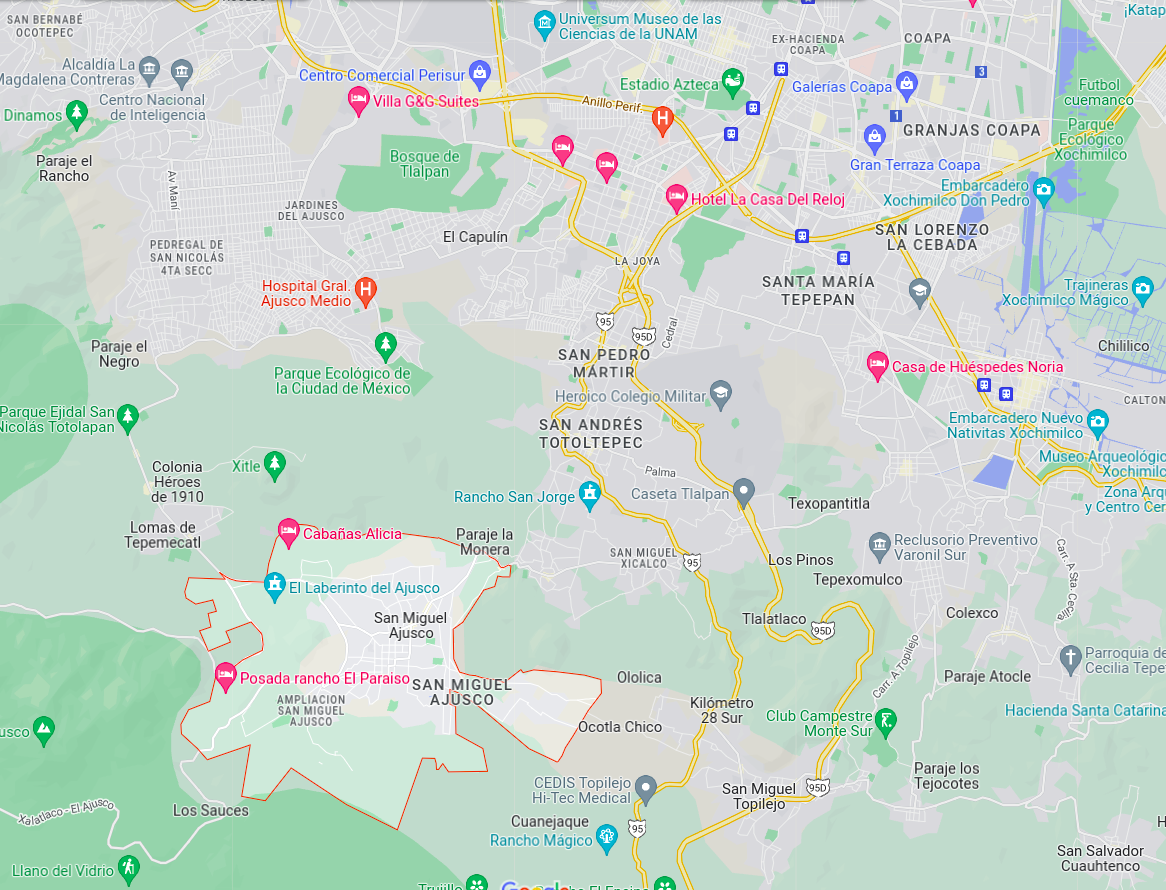
\includegraphics[scale=1]{images/cinturon_verde}
	\end{figure}
\end{frame}

\begin{frame}{Contexto}\small
	\begin{itemize}
		\item Ubicar el mejor polígono dentro de las localidades utilizando el \textbf{índice de aptitud habitad (HSI)}, que es una técnica para la toma de decisiones sobre el uso de la tierra teniendo en cuenta los requerimientos de hábitat de las especies
		\item \textbf{Análisis de sensibilidades}, determinar la sensibilidad de los hábitats presentes en una región, a través de parámetros biológicos y/o ecológicos que reflejen su grado importancia. 	
		\item Una vez determinando el mejor sitio se en las zonas propuestas se fortalecerá el proceso de gobernanza con los ejidatarios o comuneros cooperantes.
	\end{itemize}
\end{frame}

\begin{frame}{Contexto}\small

	\begin{itemize}
		\item Con estos acuerdos se realizarán acciones para determinas zonas de conservación ya sea en una UMA o ADVC para construir las instalaciones (cinco naves para 20 guajolotes cada una) con sus accesorios necesarios para realizar la etapa I que es la adaptación y manejo del guajolote en los corrales. 
		\item En esta etapa aún no se llegará a la liberación de los guajolotes.
	\end{itemize}

\end{frame}

\begin{frame}{Movebank : Eastern Wild Turkey Margadant}

	\begin{figure}
		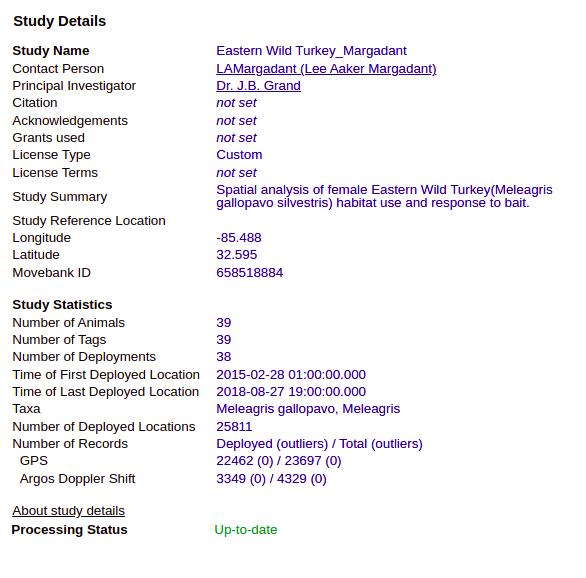
\includegraphics[scale=1.3]{images/movebank_gallopavo}
	\end{figure}
\end{frame}

\begin{frame}{Movebank : Eastern Wild Turkey Margadant}

	\begin{figure}
		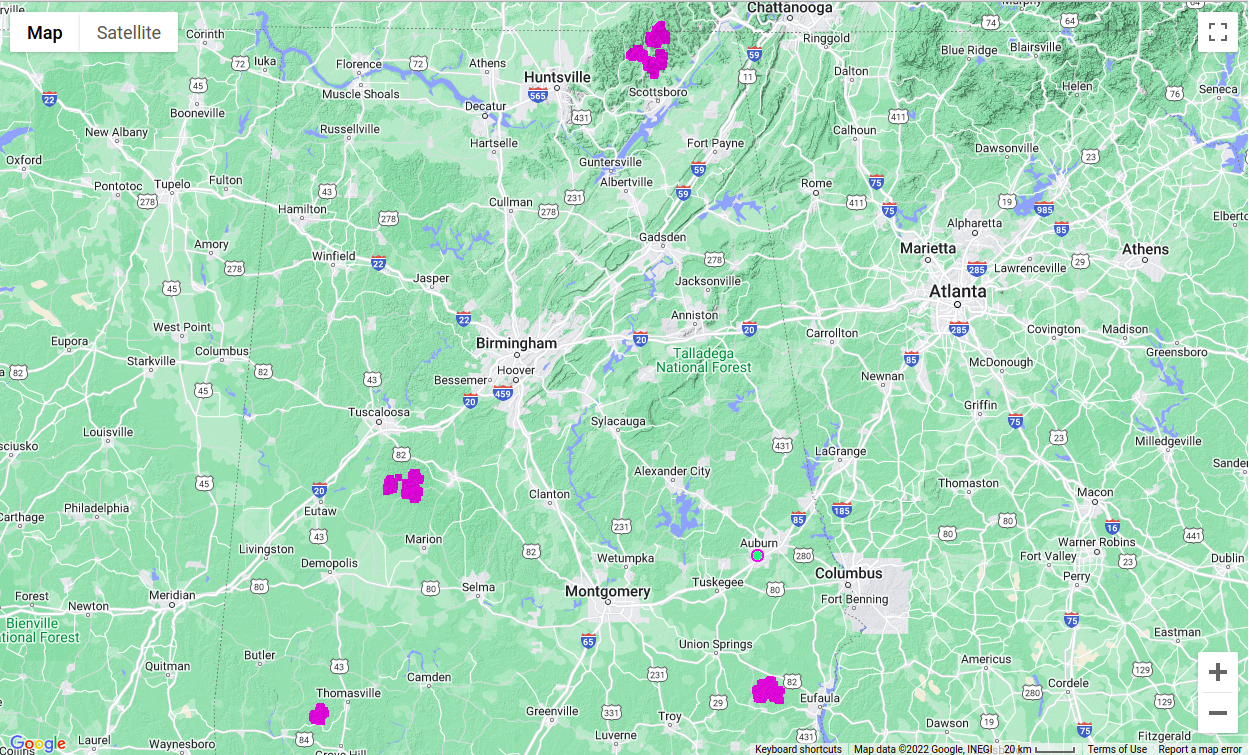
\includegraphics[scale=1]{images/movebank_gallopavo_map}
	\end{figure}
\end{frame}

\begin{frame}{Preguntas de investigación}
	\begin{itemize}
		\item ¿Cómo se modifican las áreas de actividad al considerar autocorrelación temporal y espacial de los datos?
		\item ¿Cuál es la relación entre la probabilidad de uso del paisaje y las covariables que disponemos?
		\item ¿Es posible extrapolar los resultados obtenidos de estos datos a las localidades cercanas al Ajusco-Chichinautzin del proyecto de Cinturón Verde?
	\end{itemize}
\end{frame}

\begin{frame}{Métodos}\small

	\begin{itemize}
		\item \textbf{Estimación de área de actividad con Autocorrelated Kernel Density Estimator}. El método tiene la ventaja que , además de estimar el área de actividad de los individuos, al ser un método de extrapolación, permite estimar el área de actividad que podrían utilizar los guajolotes hacia futuro. Esta caracterísitca prospectiva sería provechosa para los fines del estudio.  
		\item \textbf{Función de selección de recursos}, con el fin de obtener un mapa con las probabilidades de selección de acuerdo al paisaje, lo cual resulta provechoso para los fines de planificación y conservación asi como también para conocer la relación entre la probabilidad de uso del paisaje y las covariables.
	\end{itemize}

\end{frame}

\begin{frame}{Resultados: Autocorrelated Kernel Density Estimator}

        \begin{figure}
            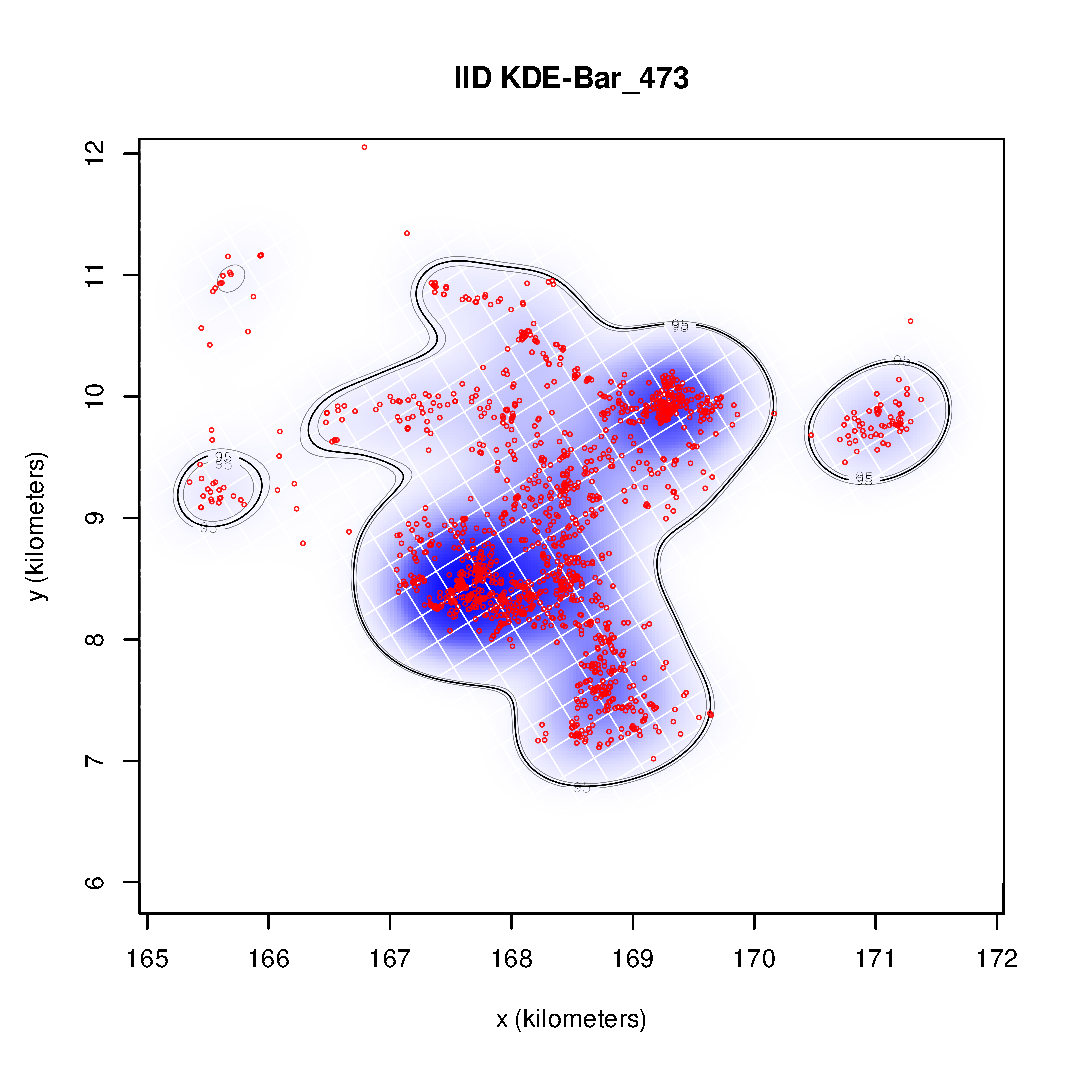
\includegraphics[scale=0.2]{images/iid_kde_Bar_473}
            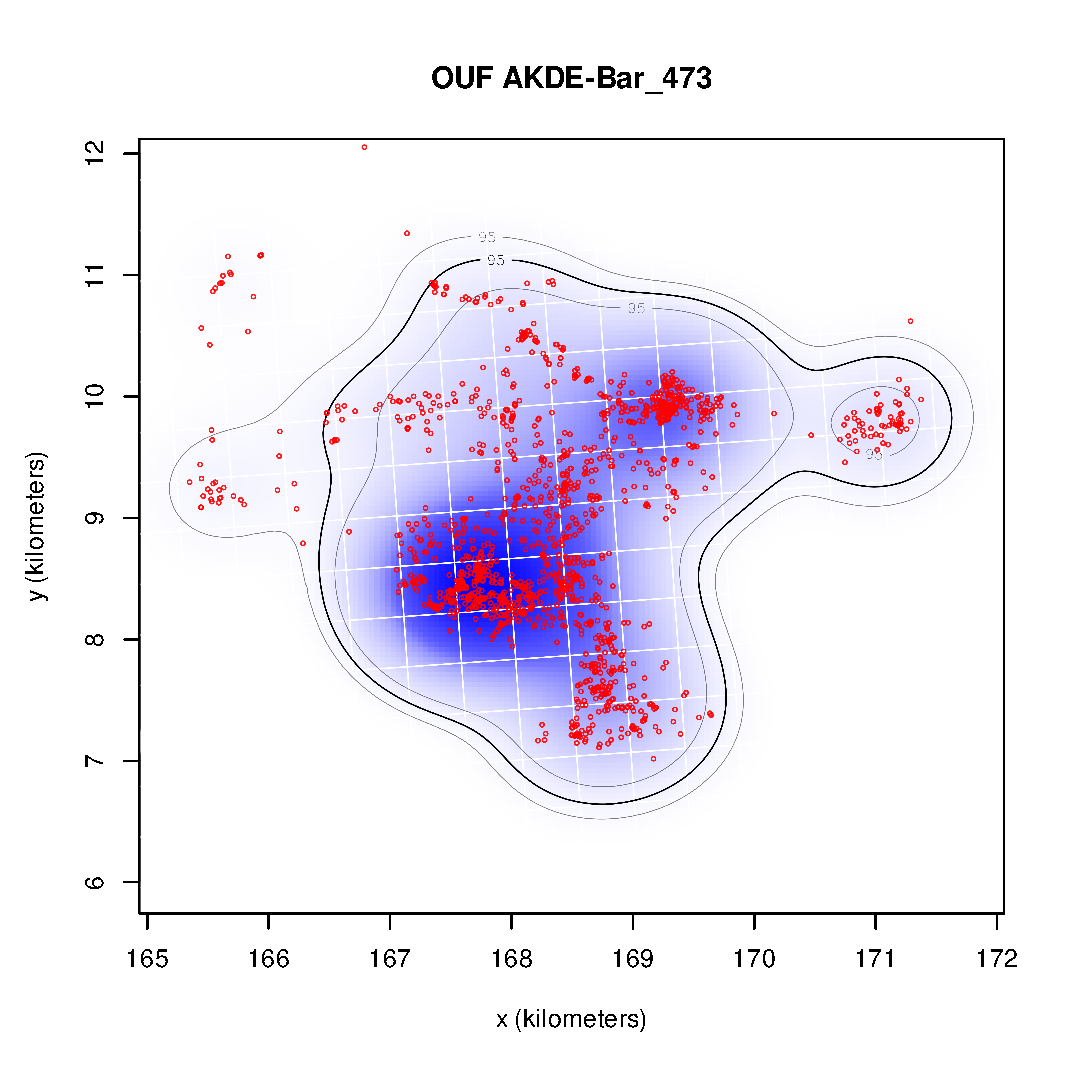
\includegraphics[scale=0.2]{images/ouf_kde_Bar_473}
            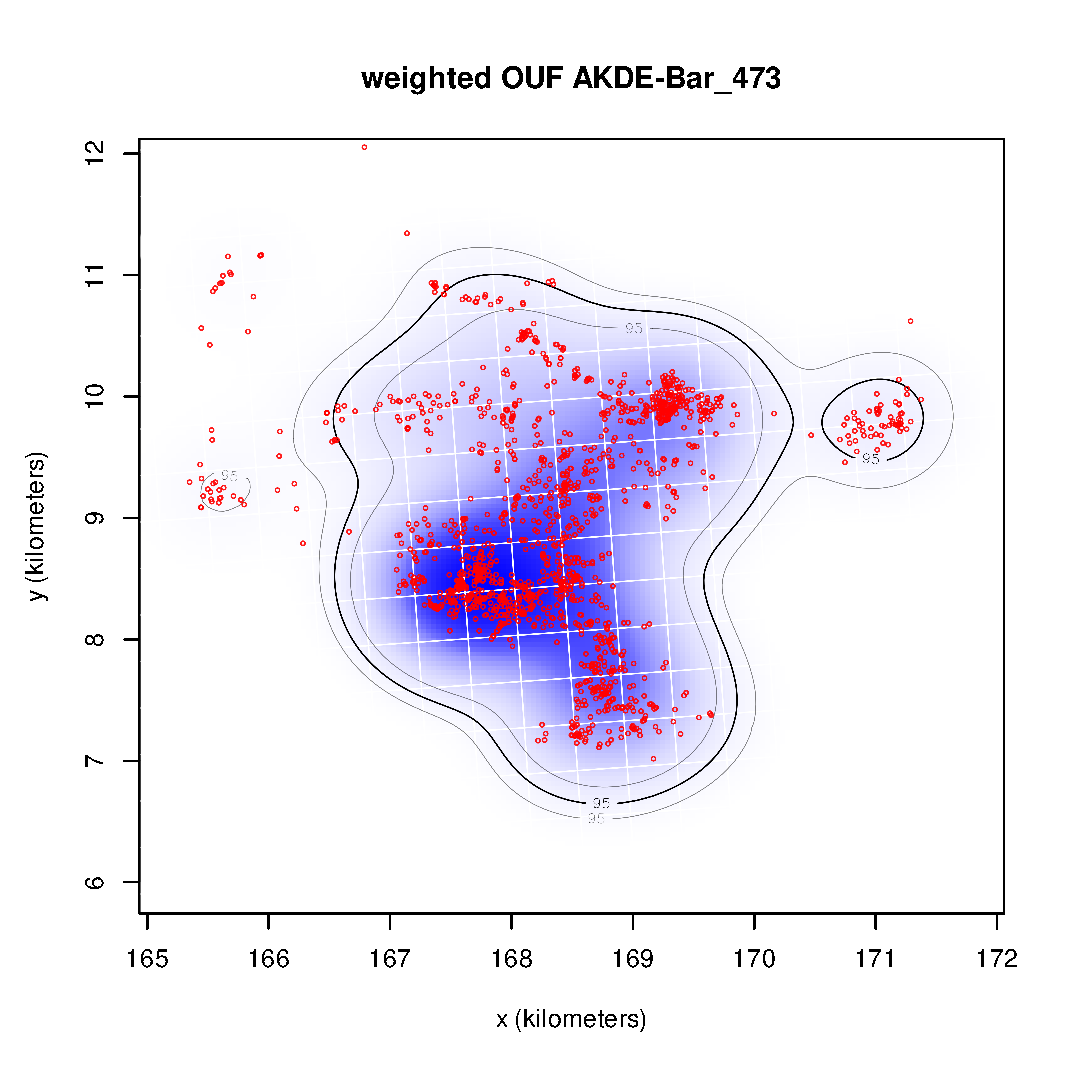
\includegraphics[scale=0.2]{images/w_ouf_kde_Bar_473}\\
            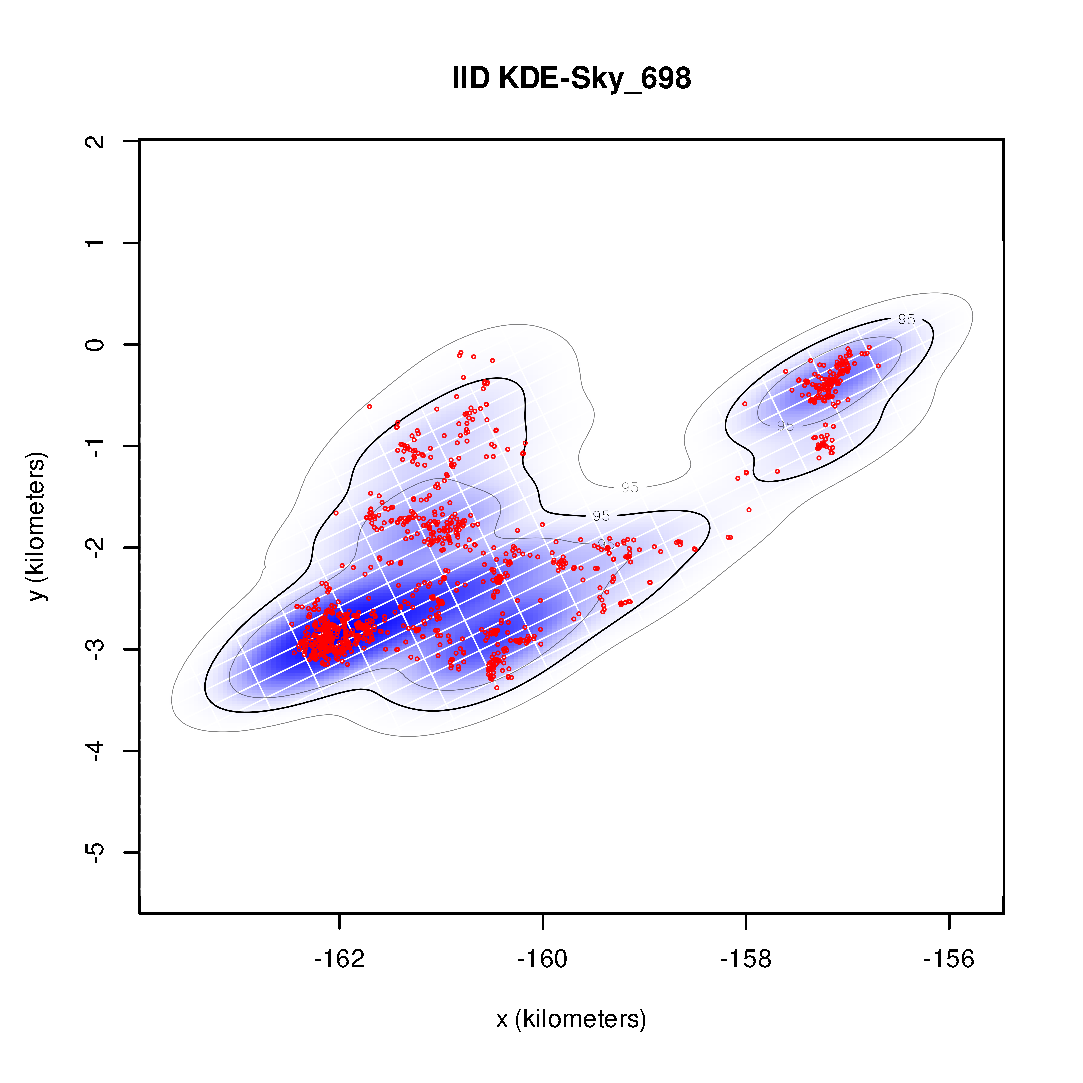
\includegraphics[scale=0.2]{images/iid_kde_Sky_698}
            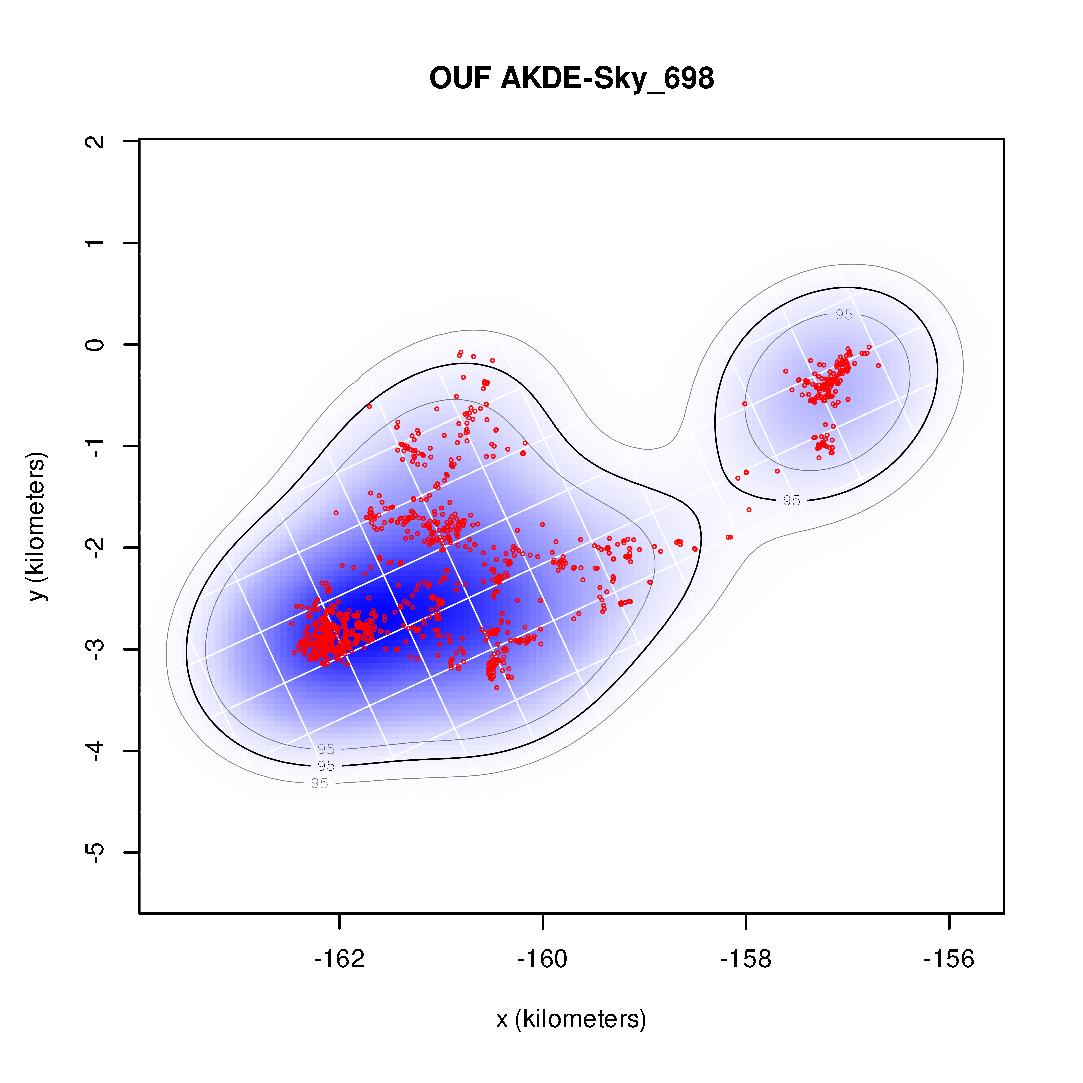
\includegraphics[scale=0.2]{images/ouf_kde_Sky_698}
            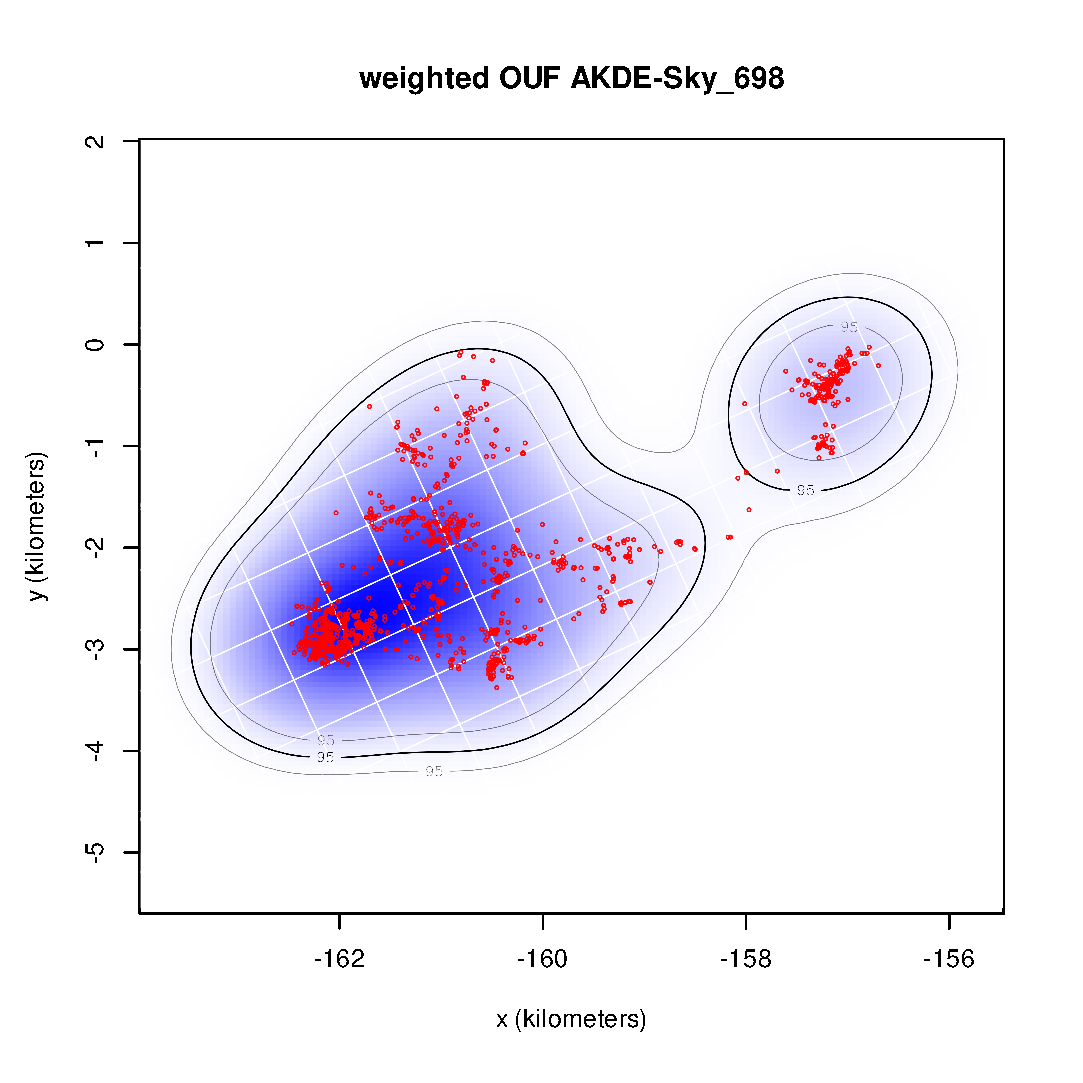
\includegraphics[scale=0.2]{images/w_ouf_kde_Sky_698}
        \end{figure}
\end{frame}



\begin{frame}{Resultados:Función de Selección de Recursos}
{ \tiny
\begin{table}[!htbp] \centering 

\begin{tabular}{@{\hspace{.01\tabcolsep}} ccccccccccc} 
\\[-1.8ex]\hline 
\hline \\[-1.8ex] 
 & (Intercept) & wetness & elevation& temperature& evi& df & logLik & AICc & delta & weight \\ 
\hline \\[-1.8ex] 

15 & 29.210 & 14.240 & -0.002 & -1.799 & 35.180 & 5 & -47,955.240 & 95,920.480 & 0 & 1 \\ 
13 & 24.990 & 18.961 &  & -1.606 & 36.511 & 4 & -48,133.540 & 96,275.080 & 354.594 & 0 \\ 
14 & 30.196 &  & -0.004 & -1.861 & 29.532 & 4 & -48,328.700 & 96,665.410 & 744.925 & 0 \\ 
10 & 21.719 &  &  & -1.482 & 28.033 & 3 & -49,029.040 & 98,064.090 & 2,143.602 & 0 \\ 
11 & 32.715 & -3.690 & -0.003 & -1.607 &  & 4 & -50,669.980 & 101,348.000 & 5,427.469 & 0 \\ 
8 & 32.339 &  & -0.002 & -1.566 &  & 3 & -50,710.270 & 101,426.500 & 5,506.060 & 0 \\ 
6& 27.737 & 1.671 &  & -1.362 &  & 3 & -50,982.710 & 101,971.400 & 6,050.927 & 0 \\ 
3 & 27.392 &  &  & -1.359 &  & 2 & -50,994.540 & 101,993.100 & 6,072.601 & 0 \\ 
12& -7.824 & 32.213 & 0.009 &  & 31.096 & 4 & -57,245.000 & 114,498.000 & 18,577.530 & 0 \\ 
5& -0.737 & 18.088 & 0.008 &  &  & 3 & -59,641.520 & 119,289.000 & 23,368.550 & 0 \\ 
9& -8.901 &  & 0.007 &  & 17.967 & 3 & -60,279.110 & 120,564.200 & 24,643.740 & 0 \\ 
2& -3.554 &  & 0.007 &  &  & 2 & -61,134.040 & 122,272.100 & 26,351.610 & 0 \\ 
7& -4.976 & 13.748 &  &  & 17.057 & 3 & -64,978.110 & 129,962.200 & 34,041.730 & 0 \\ 
4& -6.303 &  &  &  & 13.668 & 2 & -65,735.540 & 131,475.100 & 35,554.600 & 0 \\ 
1& -0.851 & 8.146 &  &  &  & 2 & -66,098.770 & 132,201.500 & 36,281.060 & 0 \\ 
\hline \\[-1.8ex] 
\end{tabular} 
  \caption{Selección de modelos} 

\end{table} 
}
\end{frame}

\begin{frame}{Resultados: Función de Selección de Recursos}

        \begin{figure}
            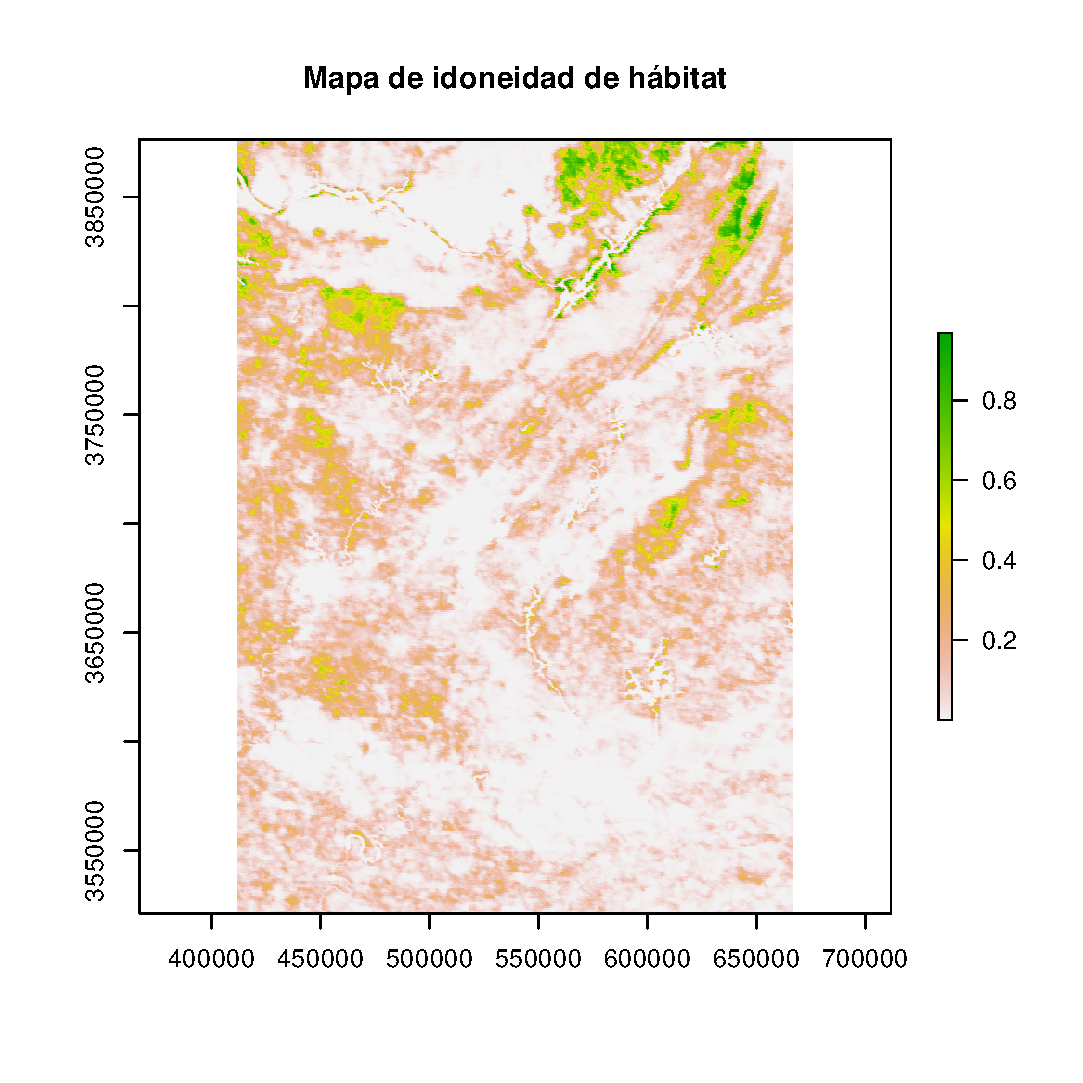
\includegraphics[scale=0.4]{images/idoneidad_habitat}
		\caption{Mapa de probabilidad de selección}
        \end{figure}
        
\end{frame}

\begin{frame}{Resultados: Función de Selección de Recursos}

        \begin{figure}
            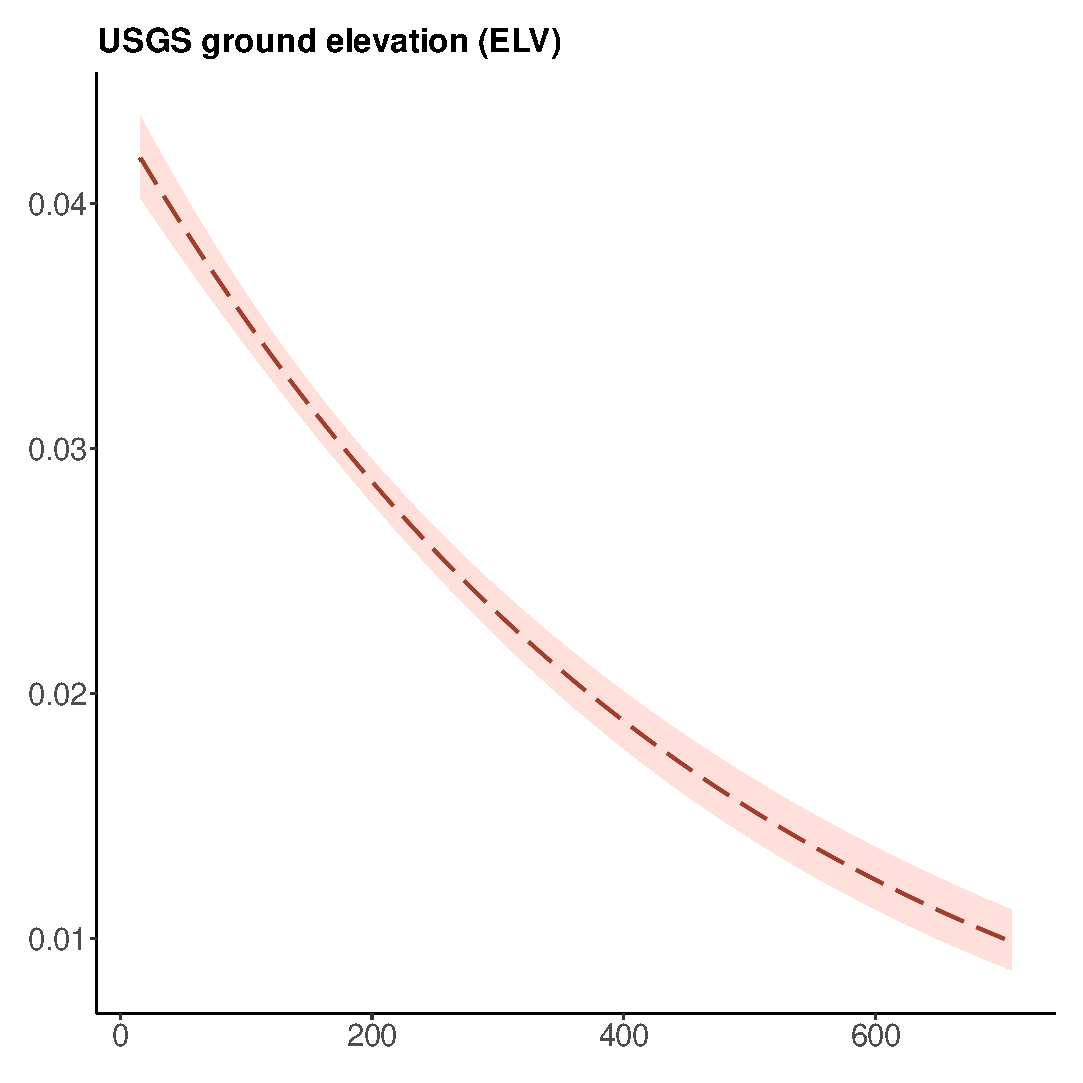
\includegraphics[scale=0.23]{images/m_effects_elevation}
            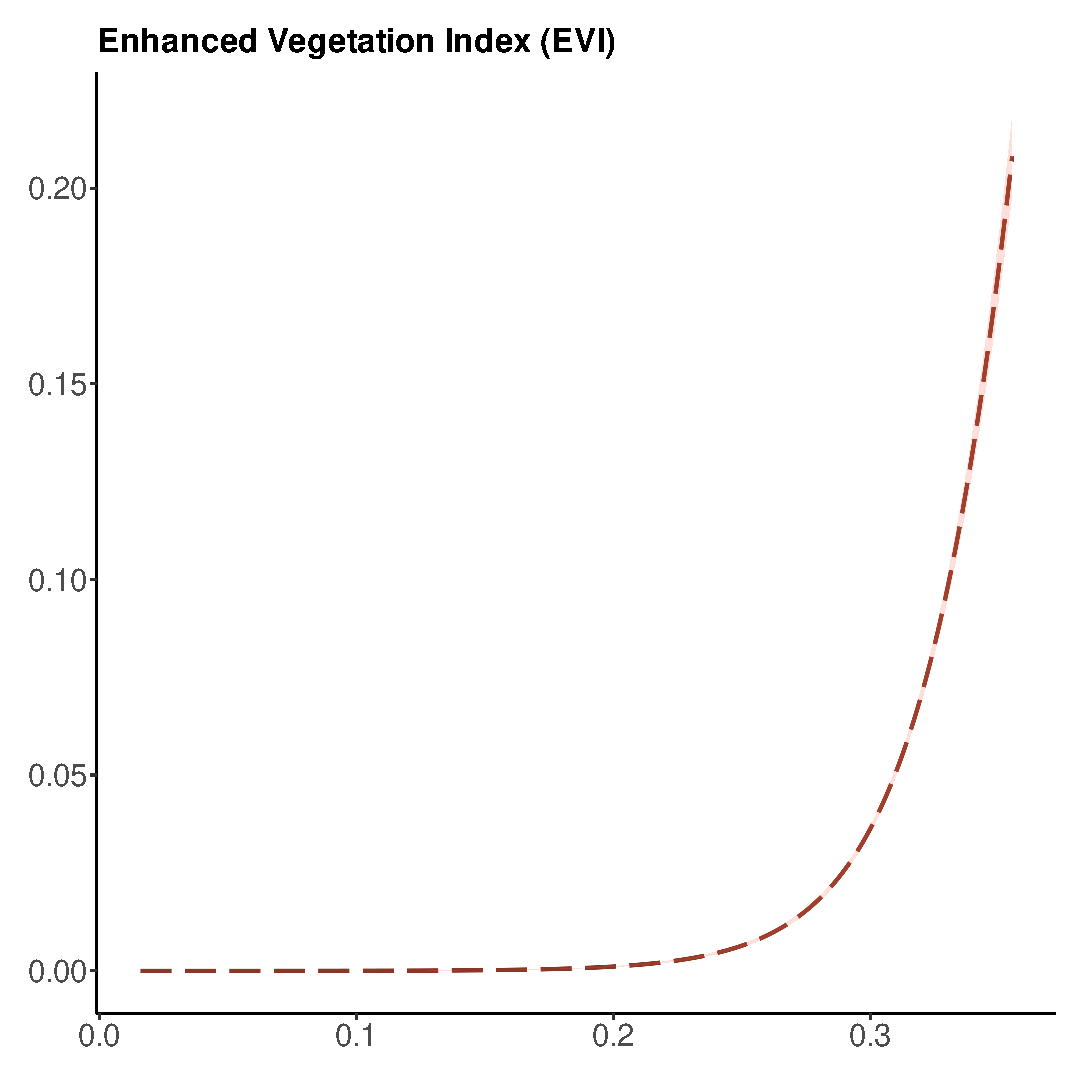
\includegraphics[scale=0.23]{images/m_effects_evi}\\
            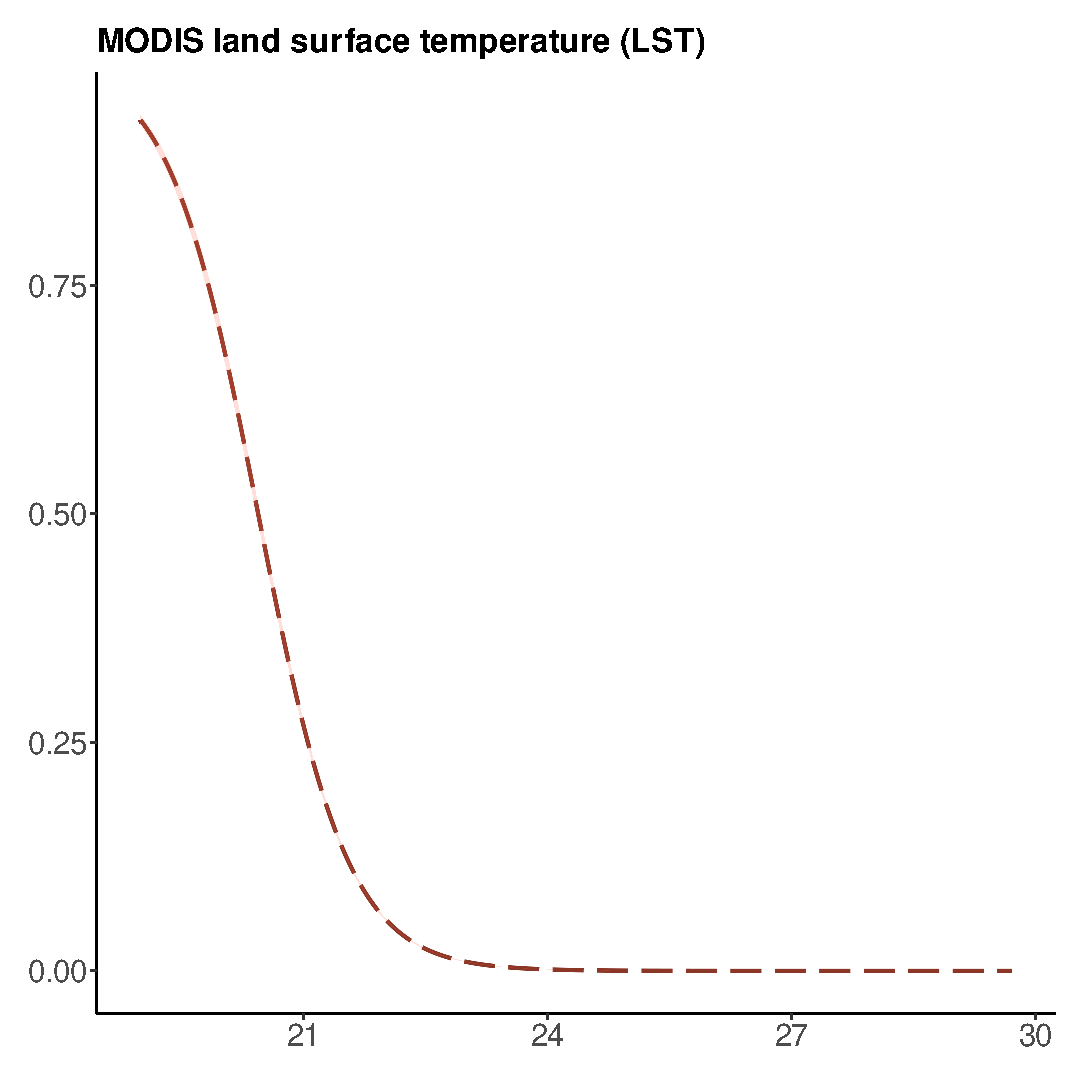
\includegraphics[scale=0.23]{images/m_effects_temperature}
            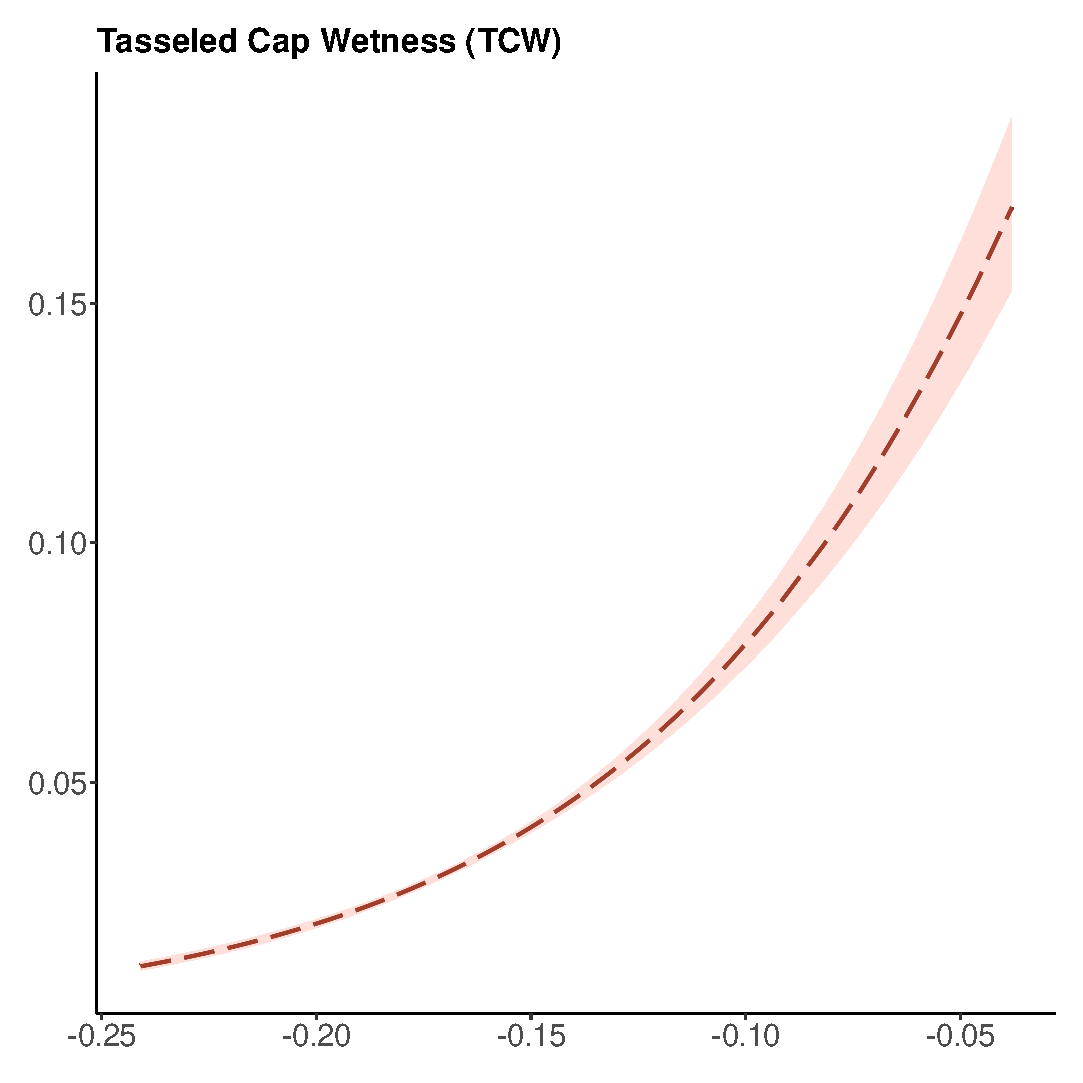
\includegraphics[scale=0.23]{images/m_effects_wetness}
        \end{figure}
\end{frame}

\begin{frame}{Conclusiones}

\end{frame}

\begin{frame}{Discusión}

\end{frame}
\end{document}